% ============================ OPERATIONS ==================================
\phase{Phase four \textbullet\ How it runs}{Operations: matching a restless supply to a steady customer}{Capacity, buffer inventory, maintenance, quality, supply chain, and a forecast of how fast India's buyers will switch.}\label{sec:ops}

Every operations problem in this plant comes from one mismatch. The refinery wants roughly the same amount of hydrogen every hour of every day. The sun shines for about a third of the day and the wind blows when it pleases. An operations manager has three ways to bridge a gap like this: hold \emph{capacity} (build more than you need), hold \emph{inventory} (store the product) or buy \emph{flexibility} (pay for a back-up). The textbook calls these the levers of aggregate planning; we use all three and let a model choose the mix.

\subsection{The dispatch model}
We wrote an hourly linear programme (a model that finds the cheapest plan meeting every constraint) for a full year of 8,760 hours. It chooses how many megawatts of solar and wind to contract, how big the hydrogen store should be, and how much firm back-up power to buy, so that the refinery gets exactly its 9,000 tonnes a year at the lowest total cost. It is solved with the HiGHS solver \cite{huangfu2018} through SciPy \cite{virtanen2020}. The solar and wind profiles here are synthetic, calibrated to typical Odisha capacity factors (solar 20.3\%, wind 33.7\%); the repository contains functions to swap in real hourly data from PVGIS and NASA POWER \cite{pvgis,nasapower}. So the shape of the answer is solid; the exact megawatts are illustrative. \confM

\begin{figure}[H]
\centering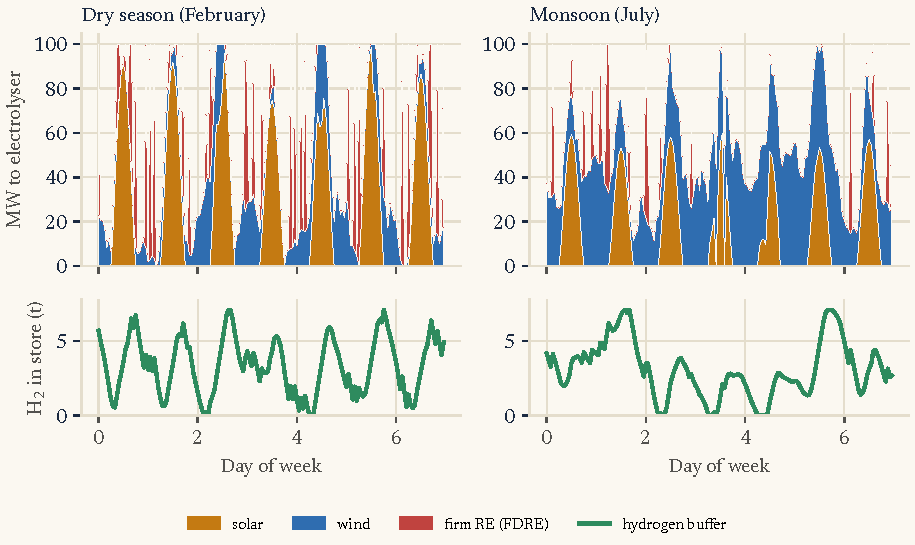
\includegraphics[width=\textwidth]{dispatch.pdf}
\caption{One week in the dry season and one in the monsoon. Top: what powers the electrolysers each hour. Bottom: tonnes of hydrogen in the buffer. Source: \texttt{dispatch.py}.}
\end{figure}

\begin{center}\tablefont
\begin{tabularx}{\textwidth}{@{}L c L@{}}
\toprule
\thead{Output} & \thead{Value} & \thead{What it means}\\ \midrule
Solar contracted & 104.7 MW & Cheap daytime energy, the bulk of supply.\\
Wind contracted & 67.8 MW & Fills evenings and the monsoon, when solar sags.\\
Renewable MW per electrolyser MW & 1.72 & We buy nearly twice the nameplate so the stack runs more hours.\\
Hydrogen buffer & 7.1 t & About 7 hours of refinery demand: safety stock, in tonnes of gas.\\
Firm back-up power share & 21.4\% & Bought at ₹5.25/kWh \cite{pvmfdre2026}: expensive, but cheaper than idle stacks.\\
Electrolyser load factor & 54.7\% & The stacks run about 4,800 full-load hours a year.\\
Renewable energy curtailed & 2.6\% & Some surplus is thrown away; storing it all would cost more.\\
Delivered power cost & \usd{}47.9/MWh & Our finance model's base uses \usd{}38; this is a cautious cross-check.\\
\bottomrule
\end{tabularx}
\end{center}

\begin{finding}[Inventory is cheaper than idle capacity, up to a point]
The model buys only about 7 tonnes of storage, because compressed hydrogen storage is expensive per tonne. It prefers to oversize the renewables and pay for some firm power. The hydrogen buffer plays the role of a classic decoupling inventory: it lets a variable upstream process feed a level downstream one. The firm power plays the role of an expedited supplier: used sparingly, at a premium. \confM
\end{finding}

\subsection{The quality constraint nobody mentions: what ``green'' allows}
India's Green Hydrogen Standard caps emissions at 2 kg of \coo{}e per kg of hydrogen, averaged over twelve months \cite{drishti2023}. India's grid emitted 0.675 kg of \coo{} per kWh in 2025--26 \cite{cea2026} \rep. At 53.2 kWh per kg, that means \textbf{grid power can supply at most about 5.6\% of our electricity} before we lose the right to call the product green, even if everything else were zero-carbon \estd.

\begin{verdict}[An operations rule that is really a compliance rule]
Our back-up power must be \emph{certified renewable} round-the-clock power, never plain grid power. If the 21\% back-up share came from the ordinary grid, our hydrogen would carry about 7.7 kg of \coo{} per kg, nearly four times the limit. Metering, hourly matching and the audit trail are therefore part of the plant's quality system, not paperwork bolted on at the end. \confH
\end{verdict}

\subsection{Maintenance and wear}
Electrolyser stacks get slowly less efficient: we assume energy use creeps up 0.6\% a year until the stack is replaced. At our load, the alkaline stacks are replaced in \textbf{year 14} and the PEM stacks in \textbf{year 11}, each costing about 35\% of a new system \estd. Two decisions follow.
\begin{itemize}
\item \textbf{A major-maintenance reserve.} Lenders do not let one year's cash flow absorb a ₹200--300 crore swap of the alkaline stacks. We set aside cash every year into a reserve account (MMRA) so the cost is spread evenly over each stack's life. In the model, this alone turned a negative cover ratio in the swap year into a smooth one.
\item \textbf{Condition-based, not calendar-based, replacement.} We monitor cell voltage stack by stack. A stack is replaced when the cost of the extra electricity it wastes exceeds the cost of carrying the new stack earlier, not when a calendar says so. This is the same logic as an economic replacement policy for any machine.
\end{itemize}

\noindent We track one headline number, borrowed from manufacturing's overall equipment effectiveness: \textbf{hydrogen effectiveness = availability $\times$ efficiency ratio $\times$ on-spec ratio}. Availability is the share of hours the plant could run; the efficiency ratio is design kWh/kg divided by actual kWh/kg; the on-spec ratio is the share of output meeting the purity and green-certification rules. It turns three separate worries into one number on the control-room wall.

\subsection{Supply chain: who we cannot afford to depend on}
We sort what we buy by how much it costs and how hard it is to replace, the Kraljic matrix of purchasing.
\begin{center}\tablefont
\begin{tabularx}{\textwidth}{@{}P{26mm} L L@{}}
\toprule
\thead{Category} & \thead{Items} & \thead{Strategy}\\ \midrule
Strategic (costly, hard to replace) & Alkaline stacks; transformers and rectifiers & Two qualified suppliers each; performance guarantees on kWh/kg and degradation; spare stack modules held on site.\\
Bottleneck (cheap, hard to replace) & Iridium-coated PEM components; membranes & Buy-back and recycling clause; a frame contract with the OEM. Iridium is the PEM's weak link \cite{h2tech2022}.\\
Leverage (costly, easy to replace) & Compressors, water treatment, pipeline & Competitive tender; standard specifications.\\
Routine & Instruments, consumables & Catalogue buying; minimum stock rules.\\
\bottomrule
\end{tabularx}
\end{center}

\subsection{Demand forecasting: how fast will Indian buyers switch?}
There is almost no past to fit a time-series model to: India's green hydrogen demand today is a few thousand tonnes. For a new product with no sales history the standard tool is the \textbf{Bass diffusion model} \cite{bass1969}, which says adoption is driven by two forces: an outside push (here, mandates, auctions and SIGHT incentives) and copying (buyers switching once they see peers do it). We let every parameter vary across a range and ran 20,000 futures. Base volumes come from the last detailed national mapping, which found about 2.6 Mt a year going into refineries out of 5.6 Mt made at home in 2018--19 \cite{igef2021}. \estd\ \confL

\begin{figure}[H]
\centering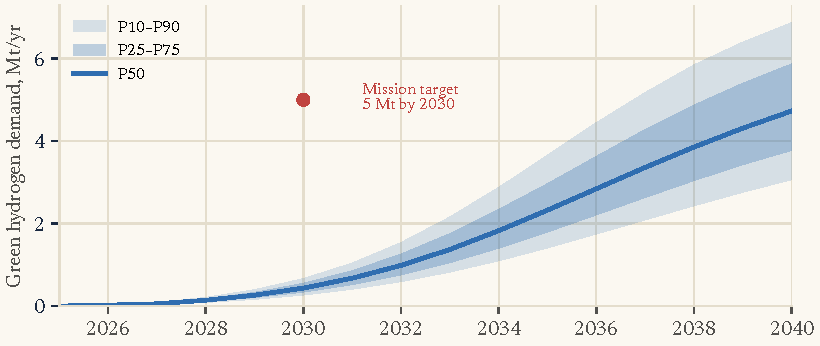
\includegraphics[width=\textwidth]{demand.pdf}
\caption{Forecast of green hydrogen demand in India, all uses, 20,000 Bass-diffusion futures. Source: \texttt{demand.py}.}
\end{figure}

\begin{center}\tablefont
\begin{tabularx}{\textwidth}{@{}L c c c@{}}
\toprule
\thead{Green hydrogen demand, Mt per year} & \thead{P10} & \thead{P50} & \thead{P90}\\ \midrule
All uses, 2030 & 0.27 & 0.44 & 0.67\\
All uses, 2035 & 1.41 & 2.32 & 3.66\\
Refining only, 2030 & 0.04 & 0.10 & 0.22\\
Refining only, 2035 & 0.20 & 0.49 & 1.02\\
\bottomrule
\end{tabularx}
\end{center}

\begin{finding}[What the forecast is for]
Two lessons, neither of which depends on the exact numbers. First, \textbf{not one of the 20,000 futures reaches the Mission's 5 million tonnes by 2030} \cite{govnow2023}; on our ranges, that target is a 2040 story. Second, our plant's 9,000 tonnes would be about \textbf{9\% of the likely green refinery market in 2030}. In a market that thin, a plant without a signed buyer is a plant without a market. Build only behind a contract. \confL\ (for the levels), \confM\ (for the lessons).
\end{finding}

\noindent Once the plant runs, forecasting becomes a different job: predicting next week's hourly power and the refinery's daily draw to plan the buffer. That calls for seasonal time-series models fed by weather forecasts; the repository's data plan (Section~\ref{sec:engine}) lists the feeds.
\newpage
